\documentclass[a4paper]{article}
\usepackage[left=1.0in, right=1.0in, top=0.4in, bottom=0.5in, includefoot, headheight=13.6pt]{geometry}
\usepackage{times}
\usepackage{tikz}
\usetikzlibrary{calc,arrows}
\parindent 0pt
\parskip 1.33ex
  
%% Begin
\title{BDI-Learning Discussion Paper \#6:\\Domain Confidence}

\author{
Dhirendra Singh\\dhirendra.singh@rmit.edu.au
}

\begin{document}

%\date{7 July 2009}

\maketitle


%%
\section*{Calculating Domain Confidence}

The motivating idea is that a confidence measure may be constructed around the rate at which new worlds are being witnessed by a plan. During early exploration it is expected that the majority of worlds that a plan is selected for will be unique, therefore this rate is high and our confidence in the resulting decision tree is low. Over time as exploration continues, the plan would get selected in all possible worlds and the rate of new worlds would taper off towards zero. Intuitively, our confidence over this period would increase to it's maximum. 

\begin{figure}[ht]
\begin{center}
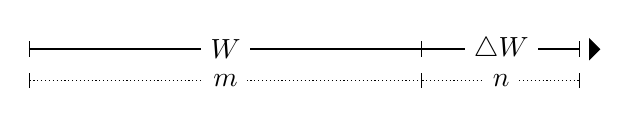
\begin{tikzpicture}
\draw[-, thick] (0,0) -- (7,0);
\draw[->,>=triangle 90] (7.25,0) -- (7.26,0);
\draw[densely dotted,|-|,>=angle 90] (0,-0.4) -- (5,-0.4) node[midway,fill=white]{$m$}; 
\draw[densely dotted,-|,>=angle 90] (5,-0.4) -- (7,-0.4) node[midway,fill=white]{$n$}; 
\draw[|-|,>=angle 90] (0,0.0) -- (5,0.0) node[midway,fill=white]{$W$}; 
\draw[-|,>=angle 90] (5,0.0) -- (7,0.0) node[midway,fill=white]{$\triangle W$}; 
\end{tikzpicture}
\end{center}
\caption{Passage of worlds with time for a given plan.}
\label{fig:domain_confidence}
\end{figure}

In inverse terms, confidence would increase with the rate at which old worlds are being witnessed. Figure \ref{fig:domain_confidence} illustrates the passage of time from the point of view of a given plan. Here $W$ is the set of all worlds witnessed in the first $m$ experiences and $\triangle W$ is the set of worlds witnessed in the last $n$ experiences. Then $|W \cap \triangle W|$ gives us the number of old worlds seen in the last $n$ experiences. Equation \ref{eqn:domain_confidence} gives the ratio that defines our confidence measure $0 \leq \kappa \leq 1.0$ that is guaranteed to converge to $1.0$ if $n<=m$ and as long as all worlds are eventually witnessed. The value $n$ may be computed as $n=a \cdot m$ where $0.0 < a \leq 1.0$ is a user-specified option.


\begin{equation}
\kappa = \frac{| W \cap \triangle W |}{n}
\label{eqn:domain_confidence}
\end{equation}


The domain confidence $\kappa$ may then be included in the calculation of the plan selection weight $\Omega(w)$ (defined in \cite{Singh:AAMAS10}) as follows:

%\begin{algorithm}[ht]
%Calculate $\Omega(w)$ from DT probability, coverage, and domain confidence\;
%\If{$\Omega <$ threshold}{
%Update $\Omega(w)$ using domain confidence measure\;
%}
%\caption{Calculation of plan selection weight $\Omega(w)$}
%\label{alg:adjust}
%\end{algorithm}

\begin{equation}
\Omega'_T(w) = 0.5 + \left[  c_T(w) *  \kappa_T * \left( p_T(w) - 0.5 \right)  \right].
\end{equation}


%%
\begin{thebibliography}{10}

\bibitem{Singh:HYCAS10}
D.~Singh, S.~Sardina, L.~Padgham.
\newblock Extending BDI Plan Selection to Incorporate Learning from Experience.
\newblock Submission under review for the Special Issue on Hybrid Control of Autonomous Systems (HYCAS), Journal of Robotics and Autonomous Systems, 2010.

\bibitem{Singh:AAMAS10}
D.~Singh, S.~Sardina, L.~Padgham, S.~Airiau.
\newblock Learning Context Conditions for {BDI} Plan Selection.
\newblock In {\em Proceedings of Autonomous Agents and Multi-Agent Systems (AAMAS)}, 2010.

\bibitem{Airiau:IJAT09}
S.~Airiau, L.~Padgham, S.~Sardina, and S.~Sen.
\newblock Enhancing Adaptation in {BDI} Agents Using Learning Techniques.
\newblock In {\em International Journal of Agent Technologies and Systems},
2009.

\end{thebibliography}

\end{document}